\documentclass[10pt]{article}
\usepackage[a4paper,left=1.45cm,right=1.45cm,top=1.1cm,bottom=1.1cm]{geometry}
\usepackage[T1]{fontenc}
\usepackage[scaled=0.95]{helvet}
\renewcommand{\familydefault}{\sfdefault}
\usepackage{microtype}
\usepackage[table]{xcolor}
\usepackage{graphicx,booktabs,tabularx,enumitem,array}
\usepackage[most]{tcolorbox}
\usepackage[hidelinks]{hyperref}
\usepackage{titlesec}

\definecolor{navy}{HTML}{1F3864}
\definecolor{accent}{HTML}{2A78D6}
\definecolor{ink2}{HTML}{52514E}
\definecolor{hair}{HTML}{C3C2B7}
\definecolor{wash}{HTML}{EEF4FC}

\titleformat{\section}{\normalsize\bfseries\color{navy}}{}{0pt}{}[{\color{hair}\titlerule}]
\titlespacing*{\section}{0pt}{1.0ex}{0.6ex}
\setlength{\parindent}{0pt}
\setlength{\parskip}{0.5ex}
\setlist{nosep,leftmargin=1.2em}
\pagestyle{empty}
\renewcommand{\arraystretch}{1.1}
\setlength{\tabcolsep}{4pt}
\newcolumntype{L}{>{\raggedright\arraybackslash}X}
\newcommand{\keyrow}[2]{#1 & \textbf{#2}\\}

\begin{document}

{\color{navy}\rule{\textwidth}{2.4pt}}\par\vspace{-0.3ex}
{\small\color{ink2}\textbf{EQUITY RESEARCH}\hfill Aerospace and defence \textbar{} London Stock Exchange\hfill 8 October 2026}\par
\vspace{-0.6ex}{\color{hair}\rule{\textwidth}{0.4pt}}\par
\vspace{0.3ex}
{\LARGE\bfseries Melrose Industries (MRO LN)}\par\vspace{0.4ex}
{\large\bfseries\color{accent}Priced as if half its profit will never turn into cash}\par\vspace{0.2ex}
{\small\color{ink2}Rohan Sharma \textbar{} MEng Design Engineering, Imperial College London}\par
\vspace{1.0ex}

\noindent
\begin{minipage}[t]{0.63\textwidth}
\vspace{0pt}
\textbf{Melrose, the owner of GKN Aerospace, is 34\% below its February high after soft guidance, a chemical incident at its Garden Grove plant and an oil spike that threatens flying hours. At 450p the market is close to valuing it as if its \emph{variable consideration} were worth nothing: engine aftermarket income it books now but collects over many years, about half of its profit. My cash flow model gives that income only partial credit and still values the shares at 609p, 35\% above the current price. I rate them BUY.}

\section{Investment thesis}
\begin{enumerate}[leftmargin=1.3em,itemsep=0.45ex]
\item \textbf{The market gives the aftermarket income almost no value.} GKN is a risk and revenue sharing partner on 19 engine families: it pays to design and make engine parts, then earns a share of each engine's sales and of decades of aftermarket revenue. Accounting rules book an estimate of that future income, called variable consideration (VC), when engines are delivered: \pounds324m in 2025, half of adjusted operating profit, none of it yet received in cash. Excluding VC, Melrose trades on 16.2x EBITDA, slightly above the 15.2x that Blackstone and Tinicum agreed to pay for UK aerospace supplier Senior plc in April. At that multiple Melrose is worth 403p if its VC is worthless and 798p if it is worth its full book value; the shares sit near the bottom of that range.
\item \textbf{Cash conversion should rise sharply.} Management targets \pounds600m of free cash flow in 2029, up from \pounds125m in 2025, as its GTF engine programmes turn cash positive in 2028 (powder-metal repair costs are expected to stay within about \pounds200m in total) and more of the aftermarket income arrives as cash. My base case reaches only 88\% of that target (at the guidance exchange rate) and still leaves 24\% of 2029 profit as non-cash VC, yet it is worth 623p a share.
\item \textbf{The setbacks are real but bounded.} I deduct \pounds120m for Garden Grove (second-half costs, a compensation fund of up to \$100m and legal costs), about 10p a share, against a \pounds2.9bn fall in market value since February. The business is still growing: in the first half of 2026, Engines revenue rose 19\% and Airframes defence sales 14\%, both at constant currency.
\end{enumerate}
\end{minipage}\hfill
\begin{minipage}[t]{0.34\textwidth}
\vspace{0pt}
\begin{tcolorbox}[colback=wash,colframe=accent,boxrule=0.8pt,arc=2pt,left=5pt,right=5pt,top=3pt,bottom=3pt]
{\Large\bfseries\color{accent}BUY}\hfill{\small\color{ink2}Fair value \textbf{\color{black}609p}}\par\vspace{0.3ex}
\small
\begin{tabularx}{\linewidth}{@{}L r@{}}
\keyrow{Price, 7 Oct 2026}{450p}
\keyrow{Upside}{+35\%}
\keyrow{Bear / base / bull}{363 / 623 / 825p}
\end{tabularx}
\end{tcolorbox}
\vspace{0.2ex}
{\small\bfseries\color{navy}Key data}\par\vspace{0.1ex}
{\footnotesize
\begin{tabularx}{\linewidth}{@{}L r@{}}
\toprule
Market value & \pounds5.6bn\\
Enterprise value, incl.\ leases & \pounds7.5bn\\
Net debt, Jun 2026 & \pounds1.53bn, 1.8x\\
P/E 2026E (peer median) & 12.9x (31.6x)\\
FCF yield 2026E (2029, \$1.37) & 3.1\% (9.8\%)\\
52-week range & 410--683p\\
Analyst targets, avg (range) & 663p (450--825p)\\
\bottomrule
\end{tabularx}}
\vspace{0.6ex}

{\small\bfseries\color{navy}Half of 2025 profit was not yet cash}\par\vspace{0.2ex}
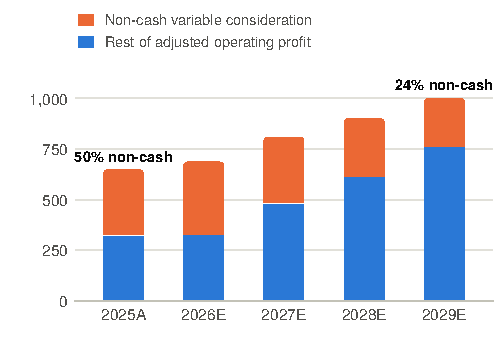
\includegraphics[width=\linewidth]{fig_profit_cash.pdf}\par
{\scriptsize\color{ink2}Adjusted operating profit, \pounds m. 2026E--29E: my base case, including the Garden Grove hit in 2026.}\par
\vspace{0.6ex}
{\footnotesize
\begin{tabularx}{\linewidth}{@{}L r r@{}}
\toprule
2025 & Revenue & Margin\\
\midrule
Engines & \pounds1,632m & 31.9\%\\
Airframes & \pounds1,957m & 8.0\%\\
Group & \pounds3,589m & 18.0\%\\
\bottomrule
\end{tabularx}}\par
{\scriptsize\color{ink2}71\% civil, 29\% defence. 2029 targets: \pounds5bn revenue, \pounds1.2bn+ profit, \pounds600m free cash flow, at \$1.25 to the pound.}
\end{minipage}

\section{What has happened}
{\small
\begin{tabularx}{\textwidth}{@{}p{1.45cm} p{1.3cm} L@{}}
19 Feb & 682.6p & 52-week high, a week before full-year results.\\
27 Feb & $-$10\% & 2026 profit guidance of \pounds700--750m misses the \pounds754m analysts expected.\\
Late May & & A chemical tank overheats at Garden Grove, one of GKN's two main window plants (cabin windows and F-35 parts); about 50,000 residents are evacuated.\\
31 Jul & 409.9p & Half-year results: the \pounds175m buyback is paused; the plant runs at about half capacity, costing about \pounds6m a month.\\
25 Aug & +8\% & A compensation fund of up to \$100m and a 28 September target for full production; no criminal charges.\\
Sep--Oct & 450p & The restart slips, pending a court-approved safety plan. Oil is back above \$100 and the 10-year gilt yield (5.48\%) is the highest since 2007.\\
\end{tabularx}}

\section{Why the low P/E is misleading}
\noindent
\begin{minipage}[t]{0.63\textwidth}
\vspace{0pt}
Melrose trades on 12.9x 2026 consensus earnings, against a 31.6x median for five aerospace peers. On that measure it looks very cheap. But its earnings include the non-cash VC: stripping it out lifts the multiple to 37.5x, above every peer except Howmet and GE Aerospace. So the shares are cheap only if the VC turns into cash. That is the question my model answers, by valuing the cash flows directly instead of applying a multiple to earnings.
\end{minipage}\hfill
\begin{minipage}[t]{0.34\textwidth}
\vspace{0pt}
{\footnotesize
\begin{tabularx}{\linewidth}{@{}L r@{}}
\toprule
P/E on 2026 consensus EPS & \\
\midrule
Howmet Aerospace & 43.4x\\
GE Aerospace & 38.3x\\
Safran & 31.6x\\
Rolls-Royce & 31.1x\\
MTU Aero Engines & 19.3x\\
\midrule
\textbf{Melrose} & \textbf{12.9x}\\
Melrose, excluding VC & 37.5x\\
\bottomrule
\end{tabularx}}\par
{\scriptsize\color{ink2}Prices 6--8 Oct 2026; S\&P Global consensus.}
\end{minipage}

\newpage
{\color{navy}\rule{\textwidth}{2.4pt}}\par\vspace{-0.3ex}
{\small\color{ink2}\textbf{Melrose Industries (MRO LN)}\hfill BUY \textbar{} Fair value 609p\hfill 8 October 2026}\par
\vspace{-0.6ex}{\color{hair}\rule{\textwidth}{0.4pt}}\par

\section{Valuation: 609p from three scenarios}
I value Melrose with a ten-year discounted cash flow model (2026--35), built division by division from the 2026 guidance mid-points and management's 2029 targets, with growth fading to 2.5\% by 2035. Non-cash VC is deducted from cash flow in full, and tax is charged at the 20.4\% adjusted rate on profit after VC. The discount rate (WACC) is 9.4\%: a 10.5\% cost of equity (10-year gilt 5.48\% plus a 5\% equity risk premium, beta 1.0) and a 5.2\% after-tax cost of debt, with debt at 21\% of capital. Value is struck at 30 June 2026, net of debt (\pounds1,530m), the pension deficit and Garden Grove costs to come.

\vspace{0.4ex}
{\small
\begin{tabularx}{\textwidth}{@{}L rrr@{}}
\toprule
 & \textbf{Bear} & \textbf{Base} & \textbf{Bull}\\
\midrule
Engines revenue growth a year, 2027--29 & 5\% & 8\% & 10\%\\
Engines margin by 2029 (2025: 31.9\%) & 32\% & 35\% & 37\%\\
Airframes growth a year, 2027--29, and margin by 2029 (2025: 8.0\%) & 3\%, 8.5\% & 5\%, 11\% & 6.5\%, 12.5\%\\
Non-cash VC as \% of Engines revenue in 2029 (2026 guidance: 20.6\%) & 16\% & 11\% & 9\%\\
Garden Grove cost still to come & \pounds250m & \pounds120m & \pounds60m\\
\midrule
2029 free cash flow (\% of management's target at \$1.37) & \pounds277m (50\%) & \pounds486m (88\%) & \pounds614m (112\%)\\
\textbf{Value per share} (change vs 450p) & \textbf{363p} ($-$19\%) & \textbf{623p} (+39\%) & \textbf{825p} (+83\%)\\
Probability & 25\% & 50\% & 25\%\\
\midrule
\multicolumn{4}{@{}l}{\textbf{Probability-weighted fair value: 609p, 35\% above the share price}}\\
\bottomrule
\end{tabularx}}

\vspace{0.5ex}
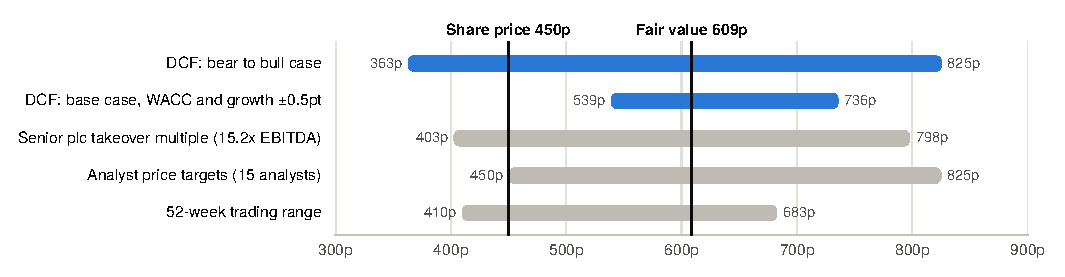
\includegraphics[width=\textwidth]{fig_football.pdf}\par
{\scriptsize\color{ink2}Valuation range by method. Blue: my model. Grey: cross-checks. The Senior bar applies its 15.2x EBITDA to Melrose's 2025 EBITDA without VC (low) and with it (high).}

\vspace{0.3ex}
\textbf{Robustness.} In the base case, all 25 combinations of WACC (8.4--10.4\%) and terminal growth (1.5--3.5\%) give a value above the share price; the lowest is 473p. The terminal value is 61\% of enterprise value and implies 8.8x 2035 EBITDA, well below the 15.2x agreed for Senior. My fair value is also below the 663p average analyst target.

\noindent
\begin{minipage}[t]{0.485\textwidth}
\section{Catalysts}
{\small
\begin{tabularx}{\linewidth}{@{}p{1.5cm} L@{}}
Q4 2026 & \textbf{Garden Grove at full output.} Ends a drag of about \pounds6m a month and could free the paused \pounds175m buyback.\\
Early 2027 & \textbf{2026 results and 2027 guidance.} First test of whether non-cash VC is falling as a share of Engines revenue.\\
End-2027 & \textbf{Airbus targets A320 output of 70--75 a month.} More engines delivered now, more aftermarket income later.\\
2028 & \textbf{GTF programmes turn cash positive.} Powder-metal repair costs (about \pounds50m in 2026) fade.\\
2029 & \textbf{\pounds600m free cash flow target.} My base case reaches 88\% of it at the \$1.37 guidance rate.\\
\end{tabularx}}

\vspace{0.6ex}
\begin{tcolorbox}[colback=white,colframe=hair,boxrule=0.5pt,arc=2pt,left=4pt,right=4pt,top=2pt,bottom=2pt]
\small\textbf{What would change my view.} If 2027 guidance shows non-cash VC still rising as a share of Engines revenue, the cash conversion case is failing and I would move to HOLD.
\end{tcolorbox}
\end{minipage}\hfill
\begin{minipage}[t]{0.485\textwidth}
\section{Risks}
{\small
\begin{itemize}[leftmargin=1em,itemsep=0.3ex]
\item \textbf{Flying hours.} With oil above \$100, airlines may cut capacity; IATA has cut its 2026 passenger growth forecast from 4.9\% to 2.1\%. Fewer flights mean fewer engine overhauls, so aftermarket cash comes later. My bear case keeps VC at 16\% of Engines revenue in 2029.
\item \textbf{Garden Grove.} At 31 July, more than 30 lawsuits and several regulatory inquiries were open and the insurance position was under review. The bear case deducts \pounds250m.
\item \textbf{Aftermarket pricing.} Management expects pricing to stay supportive ``at least in the short term''. Weaker pricing would cap Engines margins (bear case: 32\%).
\item \textbf{Interest rates.} A 0.5-point rise in the WACC cuts the base value by 56p, to 567p.
\item \textbf{Currency.} Each 1-cent move in the dollar shifts profit by about 0.7\%. I use the \$1.37 guidance rate; the pound is nearer \$1.32, which would help.
\end{itemize}}
\end{minipage}

\vfill
{\scriptsize\color{ink2}Prepared by Rohan Sharma as a personal learning project on 8 October 2026, using prices at the 7 October close. Not investment advice. Sources: Melrose FY2025 results (27 Feb 2026) and H1 2026 results (31 Jul 2026); Senior plc Rule 2.7 announcement (7 Apr 2026); lse.co.uk (prices); S\&P Global consensus via stockanalysis.com (7 Oct 2026); Trading Economics (8 Oct 2026); Reuters (25 Aug 2026); Spectrum News (28 Sep 2026); interactive investor (27 Feb 2026). Model and sources: \href{https://github.com/legend122018/melrose-valuation}{github.com/legend122018/melrose-valuation}.}

\end{document}
